% Physics of Coding Agents: Fit, Not Format at the Edit Interface
% An agent's edit is a piece that has to fit its slot in the file; fit matters more than the edit format.
\documentclass[tikz,border=0pt]{standalone}
% Shared look for the TikZ publication thumbnails.
% Canvas: 16cm x 10cm (16:10, matching the 640x400 WebP output), white, site palette.
% Labels are large (\lbl) because thumbnails are shown about 200px wide.
\usepackage[T1]{fontenc}
\usepackage{helvet}
\renewcommand{\familydefault}{\sfdefault}
\usepackage{amsmath,amssymb}
\usepackage{fontawesome5}
\usetikzlibrary{arrows.meta,calc,positioning,shapes.geometric,shapes.callouts,decorations.pathmorphing,shadows}

\definecolor{ink}{HTML}{2B2D42}
\definecolor{accent}{HTML}{B509AC}
\definecolor{teal}{HTML}{1E9BC0}
\definecolor{violet}{HTML}{6C5CE7}
\definecolor{orange}{HTML}{F28C28}
\definecolor{sun}{HTML}{F2C14E}
\definecolor{leaf}{HTML}{2CA58D}
\definecolor{alert}{HTML}{E5484D}
\definecolor{mist}{HTML}{EEF0F5}

\tikzset{
  every picture/.append style={line cap=round, line join=round},
  card/.style={rounded corners=10pt, draw=#1!75!black, line width=1.4pt, fill=#1!12},
  arrow/.style={-{Stealth[length=10pt,width=9pt]}, line width=2.2pt, draw=#1},
  soft shadow/.style={drop shadow={shadow xshift=0pt, shadow yshift=-3pt, opacity=0.18, fill=ink}},
  badge/.style={circle, fill=#1!14, draw=#1, line width=2pt, minimum size=2.3cm, text=#1},
}
\newcommand{\thumbcanvas}{\useasboundingbox[fill=white] (0,0) rectangle (16,10);}
\newcommand{\lbl}[1]{{\fontsize{20}{22}\selectfont\bfseries #1}}
\newcommand{\icon}[2][34]{{\fontsize{#1}{#1}\selectfont\faIcon{#2}}}
% Window chrome: dark editor panel with traffic-light dots. Args: x0, y0, x1, y1.
\newcommand{\editor}[4]{%
  \fill[ink, rounded corners=12pt, soft shadow] (#1,#2) rectangle (#3,#4);
  \foreach \c [count=\k] in {alert,sun,leaf} \fill[\c] ({#1+0.15+0.42*\k},{#4-0.42}) circle (0.13);
}

\begin{document}
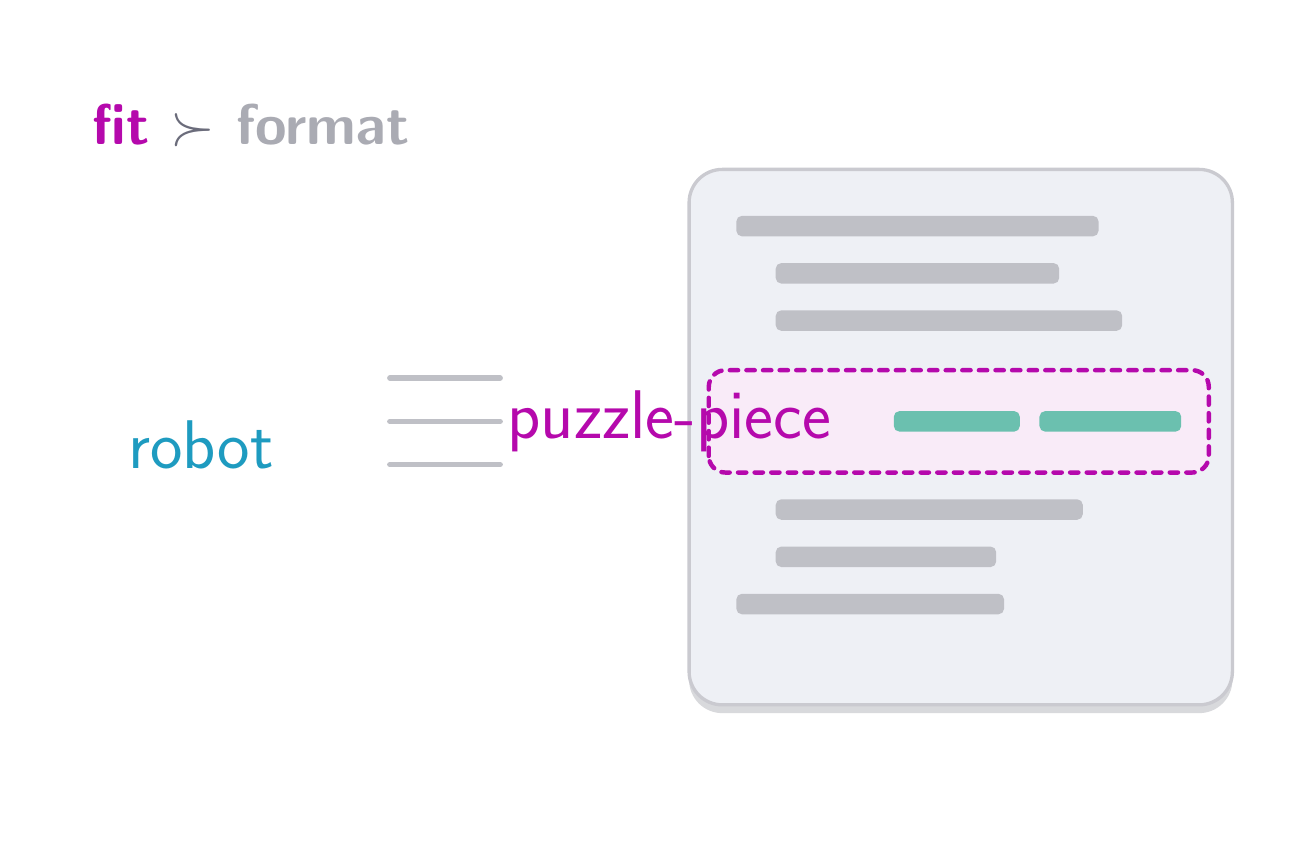
\begin{tikzpicture}
\thumbcanvas
\node[anchor=west] at (0.7,8.75) {\lbl{\textcolor{accent}{fit} \textcolor{ink!70}{$\succ$} \textcolor{ink!40}{format}}};
% The file being edited, with the slot the edit must fit.
\fill[mist, rounded corners=12pt, soft shadow] (8.4,1.4) rectangle (15.3,8.2);
\draw[ink!25, line width=1.2pt, rounded corners=12pt] (8.4,1.4) rectangle (15.3,8.2);
\foreach \y/\x/\w in {7.35/9.0/4.6,6.75/9.5/3.6,6.15/9.5/4.4,3.75/9.5/3.9,3.15/9.5/2.8,2.55/9.0/3.4}
  \fill[ink!30, rounded corners=2pt] (\x,\y) rectangle ++(\w,0.26);
\fill[accent!8, rounded corners=6pt] (8.65,4.35) rectangle (15.0,5.65);
\draw[accent, line width=1.6pt, dashed, rounded corners=6pt] (8.65,4.35) rectangle (15.0,5.65);
\foreach \x/\w in {11.0/1.6,12.85/1.8} \fill[leaf!70, rounded corners=2pt] (\x,4.87) rectangle ++(\w,0.26);
% The agent and its edit snapping into place.
\node[text=teal] at (2.2,4.7) {\icon[64]{robot}};
\foreach \y in {4.45,5.0,5.55} \draw[ink!30, line width=2pt] (4.6,\y) -- (6.0,\y);
\node[text=accent] at (8.15,5.0) {\icon[72]{puzzle-piece}};
\end{tikzpicture}
\end{document}
